\newif\ifdraft
\drafttrue
%\draftfalse

\ifdraft
  \documentclass[draft]{llncs}
  \usepackage{color}
  \usepackage[normalem]{ulem}
  \definecolor{green}{rgb}{.2,.8,0}
  \definecolor{blue}{rgb}{0,0,1}
  \definecolor{red}{rgb}{1,0,0}

  \usepackage[final]{graphicx}  
  
  \newcommand{\change}[1]{\textcolor{green}{#1}}
  \newcommand{\delete}[1]{\textcolor{red}{\sout{#1}}}
  \newcommand{\tbc}[1]{\textcolor{blue}{#1}}
  \newcommand{\todo}[1]{\textbf{\color{red}{TO-DO}}: #1}
  \newcommand{\mnote}[1]{\marginnote{#1}}
  
\else
  \documentclass{llncs}
  \usepackage{graphicx}
  
  \newcommand{\change}[1]{#1}
  \newcommand{\delete}[1]{}
  \newcommand{\tbc}[1]{#1}
  \newcommand{\todo}[1]{}
  \newcommand{\mnote}[1]{}
\fi

\usepackage{url}
\usepackage{alltt,verbatim}
\usepackage{soul}
\usepackage{subfig}
\usepackage{pifont}
\usepackage[utf8]{inputenc}

\usepackage[all]{xy}
\newcommand{\code}[1]{{\texttt{#1}}}

% MARGIN NOTES
\marginparwidth 1.25 true in

\newcounter{marginalnote}
\setcounter{marginalnote}{1}
\renewcommand{\themarginalnote}{\roman{marginalnote}}
\newcommand{\marginnote}[1]
           {\raisebox{1ex}{\scriptsize (\themarginalnote)}%
            \marginpar{\footnotesize\raggedright\indent
                       \raisebox{1ex}{\scriptsize (\themarginalnote)} #1}%
            \addtocounter{marginalnote}{1}}
% MARGIN NOTES

% Maude code
\usepackage{listings}
% Maude code

\DeclareGraphicsExtensions{.png}

\begin{document}

\pagestyle{headings} % switches on printing of running heads
%\addtocmark{XXXX} % additional mark in the TOC

\title{Solving the Movie Database Case: A solution using the Maude-based e-Motions tool.}
\titlerunning{TO-DO} % abbreviated title (for running head) also used for the TOC unless \toctitle is used

\author{Antonio~Moreno-Delgado \and Francisco~Dur\'an}
\authorrunning{Moreno et al.} %abbreviated author list (for running head)

%%%% modified list of authors for the TOC (add the affiliations)
\tocauthor{
  Antonio Moreno-Delgado (Universidad de M\'alaga),
  Francisco Dur\'an (Universidad de M\'alaga)
}

\institute{
    University of M\'alaga\\
    \email{\{amoreno,duran\}@lcc.uma.es}
    }

\maketitle

\begin{abstract}

\end{abstract}

%-------------------------------------------------------------
%  INTRODUCTION
%-------------------------------------------------------------
\section{Introduction}\label{sec:intro}

\todo{two sentences introducing Maude}

Maude may be seen as a general framework where to develop model transformations. In this way, some work has been done~\cite{troyaATL}. Since a term is very general, one could specify graphs or models as terms. Thus, a Maude module can define a \textit{in-place} model transformation, where rewriting rules define transitions between two states or models.

e-Motions~\cite{emotions} is a Domain-Specific Modeling Language (DSML) and a very general tool that supports the specification and simulation of any real-time DSML. Artifacts developed in e-Motions are translated to Maude in a transparent way. The e-Motions simulation is achieved using the Maude engine. Therefore, e-Motions can be seen as a framework where graphically code in Maude.

\subsection{e-Motions}\label{sub:emotions}
For the sake of comprehension of the rest of the paper, in this section we briefly present e-Motions. The definition of a Domain-Specific Language (DSL)\mnote{hablamos de DSLs en general, no?} comprises three tasks: (i) the definition of the abstract syntax, (ii) the definition of the concrete syntax and (iii) the specification of the behavior.

The abstract syntax is defined by means of a Ecore metamodel, in which all the language concepts and the relations between them are specified. The concrete syntax is achieved defining the so-called Graphical Concrete Syntax (GCS). A GCS is a model (conforms the GCS metamodel) where an image is attached to each concept defined in the abstract syntax.

The behavior of a DSL is specified using visual graph-transformation rules. An e-Motions rule consists of a---possibly conditional---Left-Hand Side (LHS), a Right-Hand Side (RHS) and zero or more Negative Application Conditions (NACs). The LHS defines a (sub)-graph matching, optionally conditional. The RHS specifies a (sub)-graph replacement, which if the rule is applied, every object in the LHS that is not in the RHS is deleted, new objects in the RHS that are not in the LHS are created, and those objects whose attributes (or links) are changed are updated. NACs specify conditions or (sub)-graph such that if there is a matching, the rule cannot be fired.

Fig.~\ref{fig:assemble} shows an example of an e-Motions rule.\footnote{A bunch of examples and installation help are available at \url{http://atenea.lcc.uma.es/e-Motions}.} The objects in both the RHS and LHS are represented by their images defined in the GCS model. Rule \code{Assemble}'s LHS defines the precondition of the rule. It models a assemble machine who needs both a head and a handle in its connected conveyor. If the \code{NAC1}, stating that the current matched \code{Assemble} has not unfinished other rule, is not satisfied, the rule can be applied. The rule is applied as follows. All objects in the LHS which they do not appear in the RHS are deleted, i.e. \code{he} and \code{ha} objects. Those objects in the RHS which do not appear in the LHS are created, setting their attributes properly, i.e. the \code{ham} object with its three attributes. The rest of objects remain changeless. Moreover, as e-Motions is a framework where to define real-time systems, each rule is applied in a established time, i.e. \code{[prodTime,prodTime]} in the \code{Assemble} rule. A rule may contain zero or more local or auxiliary variables. All attribute or variable assignments and conditions are coded in Object-Constraint Language (OCL)~\cite{ocl}.

The abstract and concrete syntax, and the behavior of a DSL are models and the e-Motions tool has been developed following MDE principles. The Maude code corresponding to a system defined in e-Motions is generated by an ATL/TCS transformation~\cite{atl}.

\begin{figure}[htp]
  \centering
  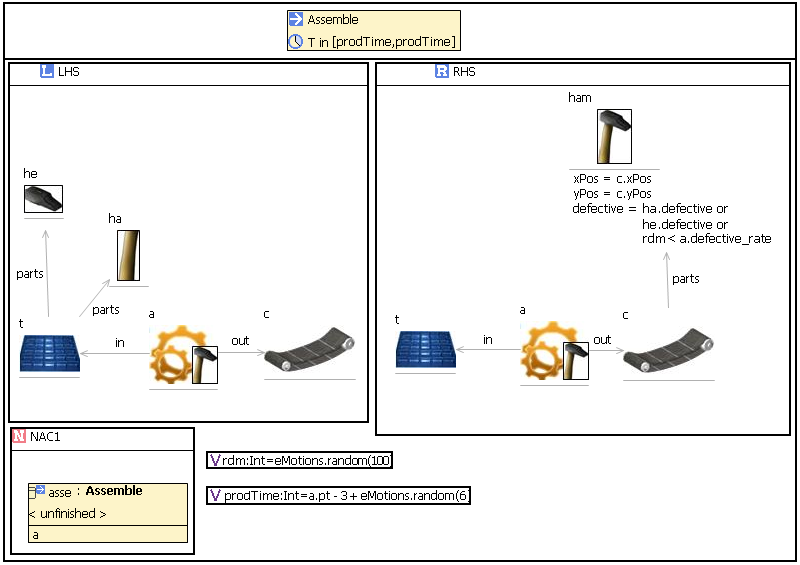
\includegraphics[width=\textwidth]{imgs/assemble}
  \caption{e-Motions \code{Assemble} rule.}\label{fig:assemble}
\end{figure}

%-------------------------------------------------------------
% SOLUTIONS
%-------------------------------------------------------------
\section{Solution}\label{sec:solution}

Since e-Motions supports in a very intuitive, user-close\mnote{esto se diría así?} and visual way, we show how the IMDb problem~\cite{imdbcase} can be solved using it. Each task is solved using the definition of a DSL, which shares in general the abstract and concrete syntax. The rewrite rules defining the behavior depends on the solution given. All rewrite rules are \textit{instantaneous}, since the case to be solved do not have time requirements.

However, e-Motions is very general: it supports OCL expressions and time requirements. This makes that the Maude code generated by e-Motions tool is not as time performance\mnote{se dice así?} as desired. Together with the e-Motions solution we present a optimized Maude solution.

\subsection{Task 1}\label{sub:task1}

Task 1 comprises the generation of synthetic models (conforming the movie database metamodel~\cite{imdbcase}) from an input parameter $N \geq 0$. Following an e-Motions based approach, we define the abstract and concrete syntax and the behavior of our so-called \textit{Task 1 DSL}, which takes a model with a parameter $N$ and generate as output a model containing synthetic data to be used as test case.

As it has been introduced in Section~\ref{sub:emotions}, the abstract syntax of a DSL is given by means of a Ecore metamodel, which is provided in~\cite{imdbsources} and, in the following, we call it \textit{Movies MM}. However, the \textit{parameter N} concept has to be modeled in some way, since in e-Motions the state\mnote{con este state me refiero al estado del sistema, de una ejecución} is just a model. Hence, a new concept call \code{Parameter} with two Integer attributes \code{nP} and \code{nN} (positive and negative graphs respectively) has been added to Movies MM. This results in a so-called \textit{Movies* MM}.\mnote{podríamos referenciar a los trabajos donde esto se hace de forma modular}

For the concrete syntax, Fig.~\ref{fig:concreteSyntax} shows how an image has been attached to each concept modeled in the Movies* MM. The behavior of this \textit{Task 1 DSL} is given by means of two in-place rules: \code{createPositive} and \code{createNegative}. Figure~\ref{fig:createPositive} shows the \code{createPositive} rule, which takes an object \code{p} of type \textit{Parameter} with \textit{nP} attribute is greater or equal than $0$ and, after the rule application, synthetic data conforming to the Henshin rules~\cite{imdbcase} are created. Fig.~\ref{fig:createNegative} shows the \code{createNegative} rule, which is analogously defined.

Once the syntax and the behavior of the system has been coded, the user may specify a model, which conforms to \textit{Movies* MM}, containing an object \code{Parameter} with its two attributes \code{nP} and \code{nN} properly set. This model is used as initial model of the execution. 

\subsubsection*{Maude version}
Concerned with the performance of e-Motions, we have specified a Maude equivalent version of Task 1. This proposal of Task 1 consists of a object-based Maude specification, which is composed by two main modules: the \code{MOVIES@MM} module defining the classes structure and the \code{TASK1} module defining the solution. The solution is coded using again two rules: \code{createPositive} and \code{createNegative}.\mnote{podriamos ponerlo en un apéndice el código} \todo{poner código con esta solución.} One could realized that the Maude version is very much like the e-Motions version. In fact, the former is just the textual version of the latter. 


\begin{figure}[htp]
  \subfloat[Actor.\label{fig:actor}]{
    \makebox[60px][c]{
\includegraphics[scale=1]{imgs/actor}}
  }
  \hfill
  \subfloat[Actress.\label{fig:actress}]{
    \makebox[60px][c]{
\includegraphics[scale=1]{imgs/actress}}
  }
  \hfill
  \subfloat[Movie.\label{fig:movie}]{
    \makebox[60px][c]{
\includegraphics[scale=1]{imgs/movie}}
  }
  \hfill
  \subfloat[Couple.\label{fig:couple}]{
    \makebox[60px][c]{
\includegraphics[scale=1]{imgs/couple}}
  }
  \hfill
  \subfloat[Parameter.\label{fig:parameter}]{
    \makebox[60px][c]{
\includegraphics[scale=1]{imgs/parameter}}
  }
  \caption{Concrete syntax for \textit{Movies* MM}.}
  \label{fig:concreteSyntax}
\end{figure}

\todo{Correctness?}

\todo{Time tables once we have installed maude in the Ubuntu image}

\begin{figure}[htp]
  \subfloat[The \code{createPositive} rule.\label{fig:createPositive}]{%
    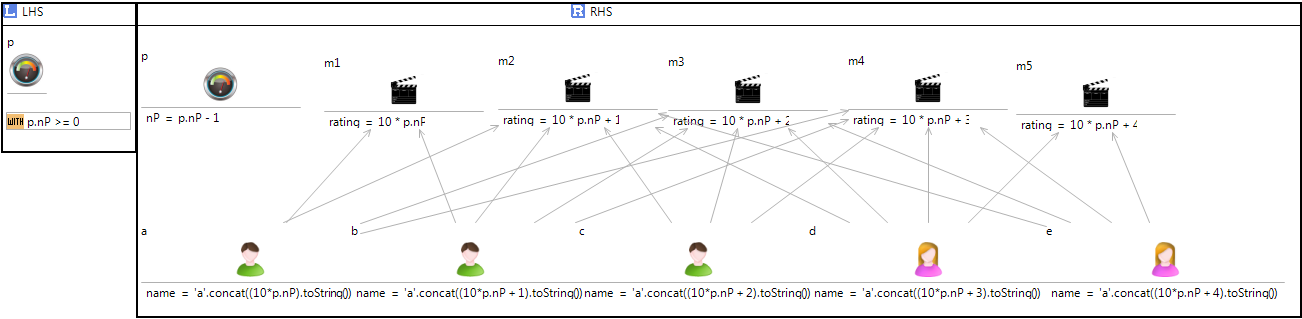
\includegraphics[width=\textheight, angle=90]{imgs/createPositiveRule}
  }
  \hfill
%  \subfloat[Rules' headers.]{
%    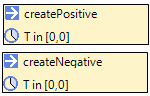
\includegraphics[width=0.2\textwidth]{imgs/headersCreate}
%  }
%  \hfill
  \subfloat[The \code{negativePositive} rule.\label{fig:createNegative}]{%
    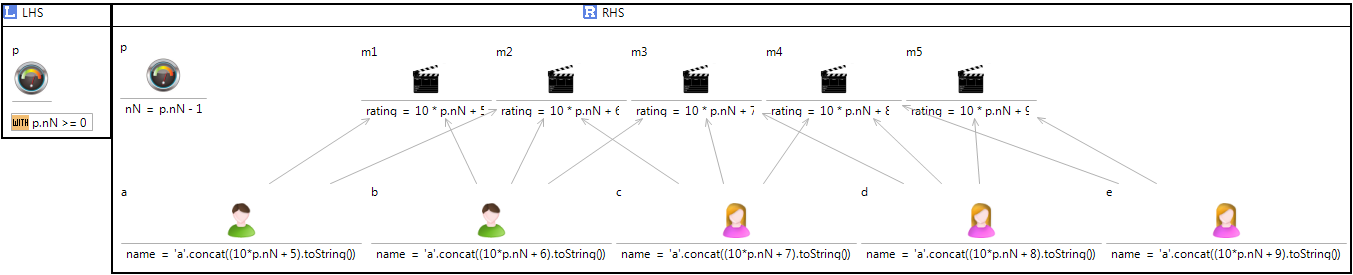
\includegraphics[width=\textheight, angle=90]{imgs/createNegativeRule}
  }
  \label{fig:task1}
  \caption{Task 1 rules.}
\end{figure}

\subsection{Task 2}
Task 2 consists of extract all couples from a given model, either from Task 1 or IMBd database~\cite{todo}. Two persons are couple whether they played together in at least three movies~\cite{imdbcase}.

Fig.~\ref{fig:createCouple} shows the \code{createCouple} rule which implements this task. The \code{createCouple} rule consists of a LHS with a OCL condition, which states \textit{``LHS holds iff there are two persons \code{per1} and \code{per2}, such that the number of movies in the intersection between \code{per1}'s movies and \code{per2}'s movies is greater or equal than 3''}. Moreover, the \code{coupleHasNotBeenCreated} NAC avoids the application of the rule if the couple already exists. 

\begin{figure}[htp]
  \centering
  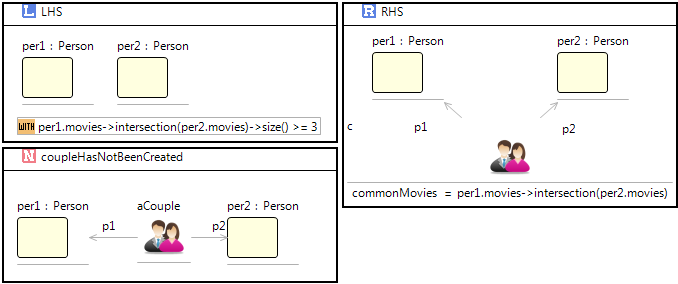
\includegraphics[width=\textwidth]{imgs/ruleCouples}
  \caption{\code{createCouple} rule.}\label{fig:createCouple}
\end{figure}

\bibliographystyle{splncs03}
\bibliography{TTC14}
\providecommand{\url}[1]{\texttt{#1}}
\end{document}
